
\chapter{Finite Element Volume Method}
\label{chp:HFVMMethod}
%introduction

%Point back to goals of a method
%Requires use of a FEM and a FVM
% FVM was shown to work previously [hank,Zoppou] 

%update method
\cite{Pitt-2018-61}





%describe grids up here

\section{Notation for Numerical Grids}
We begin by defining the numerical grid in both space and time from a starting location $x_0$ and a beginning time $t^0$. For any $j,n \in \mathbb{N}$ we have
\begin{subequations}
\begin{align}
x_j &= x_0 + j \Delta x,  \\
t^n &= t^0 + n \Delta t
\end{align}
\label{eqn:NumGridDef}
\end{subequations}
which produces a uniform grid; $x_j$ in space and $t^n$ in time. The Finite Element Volume Method (FEVM) can be readily adapted to nonuniform grids and we restrict our description of the method to uniform grids for simplicity. This notation is extended to locations and times not on the grid using subscripts and superscripts in $\mathbb{R}$ for \eqref{eqn:NumGridDef}.

The grid notation naturally extends to our quantities of interest, for example, for a general quantity $q$
\begin{equation}
q^n_j = q(x_j ,t^n). 
\end{equation}
This applies for all subscripts and superscripts in $\mathbb{R}$. Throughout the rest of this Thesis $j$ and $n$ will be used exclusively to denote general locations on the grid and thus are members of $\mathbb{N}$.

%cells
The description of our numerical method focuses on cells which are regions surrounding the grid points. The $j^{th}$ cell is the region $\left[x_{j - 1/2} , x_{j + 1/2}\right]$ centred around $x_j$. For each cell we define the average of a quantity
\begin{equation}
\overline{q}_j = \frac{1}{\Delta x} \int_{x_{j-1/2}}^{x_{j+1/2}} q(x,t) \; dx
\end{equation}
in cell $j$.

In the FEVM we reconstruct quantities at various points inside the cell from the cell average values. We distinguish between two reconstructions that are possible at each cell edge, which exist due to the overlap of neighbouring cells. To do this we use superscripts so that for the cell edge $x_{j+1/2}$ and a general quantity $q$, we have $q^-_{j+1/2}$ as the reconstructed value of $q$ at $x_{j+1/2}$ from the $j^{th}$ cell and $q^+_{j+1/2}$ as the reconstructed value of $q$ at $x_{j+1/2}$ from the $(j+1)^{th}$ cell. Since the particular time level is typically obvious from context and hence omitted the use of a superscript will not clutter the notation.

\section{Structure Overview}
\label{sec:StructOverview}
%define w,b
To describe the FEVM we first present an overview of the evolution step and then provide the details for each component. We begin our evolution step with all the cell averages for $h$, $w$ and $G$ at time $t^n$ and all the nodal values of $b$. We write these as vectors from the $0^{th}$ cell to the $m^{th}$ in the following way
\begin{align*} \overline{\vecn{h}} = \begin{bmatrix}
\overline{h}_0^n \\\overline{h}_1^n \\ \vdots \\ \overline{h}_m^n \end{bmatrix} &,& \overline{\vecn{w}} = \begin{bmatrix}
\overline{w}_0^n \\\overline{w}_1^n \\ \vdots \\ \overline{w}_m^n \end{bmatrix} &,&  \overline{\vecn{G}} = \begin{bmatrix}
\overline{G}_0^n \\\overline{G}_1^n \\ \vdots \\ \overline{G}_m^n \end{bmatrix}& &\text{and}& & \vecn{b} = \begin{bmatrix}
b_{0} \\ b_{1} \\ \vdots \\b_{m}
\end{bmatrix}. \\
\end{align*}
The evolution step proceeds as follows:
\begin{enumerate}[(i)]
	\item Reconstruction: We reconstruct the quantities $h$, $w$, $G$ and $b$ inside every cell at various points, which are demonstrated for the $j^{th}$ cell in Figure \ref{fig:ReconLocs}. The values of $h$, $w$ and $G$ in the $j^{th}$ cell are reconstructed at $x_{j-1/2}$, $x_{j}$ and $x_{j+1/2}$ using the reconstruction operators $\mathcal{R}^+_{j-1/2}$, $\mathcal{R}_{j}$ and $\mathcal{R}^-_{j+1/2}$ respectively. The bed profile $b$ in the $j^{th}$ cell is reconstructed at $x_{j-1/2}$, $x_{j-1/6}$, $x_{j+1/6}$ and $x_{j+1/2}$ using the reconstruction operators $\mathcal{B}_{j-1/2}$, $\mathcal{B}_{j-1/6}$, $\mathcal{B}_{j+1/6}$ and $\mathcal{B}_{j+1/2}$ respectively. So that
	\begin{align*}	&h^+_{j-1/2} = \mathcal{R}^+_{j-1/2} \left(\overline{\vecn{h}}\right),&& G^+_{j-1/2} = \mathcal{R}^+_{j-1/2} \left(\overline{\vecn{G}}\right),\\
	&h_j = \mathcal{R}_{j} \left(\overline{\vecn{h}}\right),&& G_j = \mathcal{R}_{j} \left(\overline{\vecn{G}}\right),\\
	&h^-_{j+1/2} = \mathcal{R}^-_{j+1/2}\left(\overline{\vecn{h}}\right),&& G^-_{j+1/2} = \mathcal{R}^-_{j+1/2} \left(\overline{\vecn{G}}\right),\\ \\
	&w^+_{j-1/2} = \mathcal{R}^+_{j-1/2} \left(\overline{\vecn{w}}\right), &&b_{j-1/2} = \mathcal{B}_{j-1/2} \left(\vecn{b}\right),  \\
	&w_{j} = \mathcal{R}_{j} \left(\overline{\vecn{w}}\right), &&b_{j-1/6} = \mathcal{B}_{j-1/6}  \left(\vecn{b}\right),\\
	&w^-_{j+1/2} = \mathcal{R}^-_{j+1/2} \left(\overline{\vecn{w}}\right), &&b_{j+1/6} = \mathcal{B}_{j+1/6} \left(\vecn{b}\right), \\
	& && b_{j+1/2} = \mathcal{B}_{j+1/2}  \left(\vecn{b}\right).\\
	\end{align*}
	This generates the vectors of these quantities reconstructed for every cell; $\vecn{\hat{h}}$, $\vecn{\hat{w}}$, $\vecn{\hat{G}}$ and $\vecn{\hat{b}}$ which are
	\begin{align*}\vecn{\hat{h}} = \begin{bmatrix}
	h^+_{-1/2} \\ h_0 \\ h^-_{1/2} \\ h^+_{1/2}  \\ \vdots \\ h_m \\ h^-_{m+1/2}\end{bmatrix} &,&
	\vecn{\hat{w}} = \begin{bmatrix}
	w^+_{-1/2} \\ w_0 \\ w^-_{1/2} \\ w^+_{1/2}  \\ \vdots \\ w_m \\ w^-_{m+1/2}\end{bmatrix} &,& \vecn{\hat{G}} = \begin{bmatrix}
	G^+_{-1/2} \\ G_0 \\ G^-_{1/2} \\ G^+_{1/2}  \\ \vdots \\ G_m \\ G^-_{m+1/2}
	\end{bmatrix} & &\text{and}& & \vecn{\hat{b}} = \begin{bmatrix}
	b_{-1/2} \\ b_{-1/6} \\ b_{1/6} \\ b_{1/2} \\ \vdots \\ b_{m + 1/6}\\ b_{m+1/2}
	\end{bmatrix}.
	\end{align*}
	
	\item Fluid Velocity: The remaining unknown quantity, the depth averaged fluid velocity $u$ is calculated by solving the elliptic equation \eqref{defn:SerreEqnConservedQuantity1} with a Finite Element Method (FEM) from which we obtain $u_{j-1/2}$, $u_j$ and $u_{j+1/2}$ for every cell. We denote the solution of the FEM by the map $\mathcal{G}$ given  $\vecn{\hat{h}}$, $\vecn{\hat{G}}$ and $\vecn{\hat{b}}$ as inputs. So that
	\begin{equation*}
	\vecn{\hat{u}} = 
	\begin{bmatrix}
	u_{-1/2} \\ u_0 \\ u_{1/2} \\ \vdots \\ u_m \\ u_{m+1/2}
	\end{bmatrix} = \mathcal{G}\left( \vecn{\hat{h}}, \vecn{\hat{G}},\vecn{\hat{b}} \right).
	\end{equation*}
	\item Flux Across Cell Interfaces: We calculate the average fluxes $F_{j-1/2}$ and $F_{j+1/2}$ across the cell boundaries $x_{j-1/2}$ and $x_{j+1/2}$ over time using $\mathcal{F}_{j-1/2}$ and $\mathcal{F}_{j+1/2}$ so that
		\begin{align*}	
		F_{j-1/2} &=\mathcal{F}_{j-1/2} \left( \vecn{\hat{h}}, \vecn{\hat{G}},\vecn{\hat{b}}, \vecn{\hat{u}}  \right),\\
		F_{j+1/2} &=\mathcal{F}_{j+1/2} \left(\vecn{\hat{h}}, \vecn{\hat{G}},\vecn{\hat{b}}, \vecn{\hat{u}}  \right).
		\end{align*}
	\item Source Terms: We calculate the source term contribution to the cell average of a quantity over a time step $S_{j}$ with the operator $\mathcal{S}$ like so
	\begin{equation*}	
	S_{j} =\mathcal{S}_{j} \left( \vecn{\hat{h}},\vecn{\hat{w}},\vecn{\hat{b}}, \vecn{\hat{u}}  \right).
	\end{equation*}
	\item Update All the Cell Averages Using a Forward Euler Approximation: We update the cell average values from time $t^n$ to the next time level combining a forward Euler approximation and a fractional step method for the flux and source terms.
	\item Update All the Cell Averages Using a Second-Order SSP Runge-Kutta Method: We repeat steps (I)-(V) and use SSP Runge-Kutta time stepping to calculate $\overline{\vecn{h}}$ and $\overline{\vecn{G}}$ at $t^{n+1}$ with second-order accuracy in space and time.
\end{enumerate}

\setcounter{subsection}{0}
\renewcommand{\thesubsection}{(\roman{subsection})} 
\subsection{Reconstruction}
We now provide the details for the reconstruction of $h$, $w$, $G$ and $b$ in the $j^{th}$ cell at the locations demonstrated in Figure \ref{fig:ReconLocs}. For $h$, $w$ and $G$ the reconstructions is performed from the cell averages. While $b$ is reconstructed from the nodal values.

\begin{figure}
	\centering
	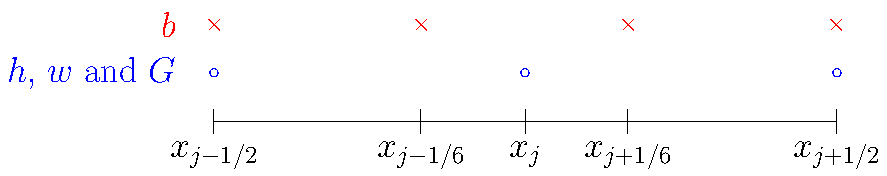
\includegraphics[width=0.8\textwidth]{./chp3/figures/FEVMRecon.pdf}
	\caption{Location of the reconstructions for $h$, $w$, $G$ and $b$ inside the $j^{th}$ cell.}
	\label{fig:ReconLocs}
\end{figure}

\subsubsection{The height, stage and $G$}
We reconstruct $h$, $w$ and $G$ with piecewise functions that are linear over a cell and discontinuous at the cell edges. Since $h$, $w$ and $G$ use the same reconstruction operators we demonstrate them for a general quantity $q$. For the $j^{th}$ cell we reconstruct the values of $q$ at $x_{j-1/2} $, $x_{j} $ and $x_{j+1/2}$ in the following way
%cite someone 
\begin{subequations}
	\begin{align}
	q^+_{j-1/2} & = \mathcal{R}^+_{j-1/2} \left(\overline{\vecn{q}}\right) = \bar{q} - \dfrac{\Delta x}{2} d_j, \\
	q_{j} &= \mathcal{R}_{j} \left(\overline{\vecn{q}}\right) =\bar{q} ,\\
	q^-_{j+1/2} &= \mathcal{R}^-_{j+1/2} \left(\overline{\vecn{q}}\right) = \bar{q} + \dfrac{\Delta x}{2} d_j
	\end{align}
	\label{eqn:ReconforhwG}
\end{subequations}
where 
\begin{equation}
d_j = \text{minmod}\left(\theta \dfrac{\overline{q}_j -\overline{q}_{j-1} }{\Delta x}, \dfrac{\overline{q}_{j+1} -\overline{q}_{j-1} }{2\Delta x}, \theta\dfrac{\overline{q}_{j+1} -\overline{q}_{j} }{\Delta x}\right)
\label{eqn:slopehGrecon}
\end{equation}
with $\theta \in \left[1,2\right]$. The choice of the $\theta$ parameter changes the diffusion introduced by the reconstruction, with $\theta =1$ the reconstruction introduces the most diffusion and is equivalent to the minmod reconstruction \cite{Roe-1986-337}. When $\theta = 2$ the reconstruction introduces the least diffusion and is equivalent to the monotized central reconstruction \cite{VanLeer-1977-276}.

\begin{defn}
The minmod function takes a list of $a_i \in \mathbb{R}$. If all elements have the same sign then minmod returns the element with smallest absolute value, otherwise it returns $0$. 
	\begin{equation*}
	\text{minmod}\left(a_0,a_1,\dots\right) := \left\lbrace \begin{array}{l l}
	\min\left\lbrace a_i\right\rbrace & a_i > 0 \; \forall i \\
	\max\left\lbrace a_i\right\rbrace & a_i < 0  \; \forall i \\
	0 & \text{otherwise}\\
	\end{array} \right. . 
	\end{equation*}
\end{defn}
The nonlinear limiting used to calculate $d_j$ ensures that the reconstruction of $h$, $w$ and $G$ inside the cell is Total Variation Diminishing (TVD), hence it does not introduce non-physical oscillations. The TVD property is attained by constraining the slope $d_j$ to zero near local extrema, resulting in a first-order approximation which is necessarily TVD. Away from local extrema $d_j$ will be the gradient with the smallest absolute value, making our reconstruction second-order accurate.

The reconstruction operator $\mathcal{R}_{j} $ is second-order accurate regardless of the presence of local extrema. This can be seen through the error analysis of the midpoint quadrature rule for which we have that
\begin{equation}
\overline{q} = \frac{1}{\Delta x} \int_{x_{j-1/2}}^{x_{j+1/2}} q \; dx = q_j + \mathcal{O}\left(\Delta x^2\right).
\end{equation}

\subsubsection{The bed profile}
To reconstruct $b$ at $x_{j-1/2}$, $x_{j-1/6}$, $x_{j+1/6}$ and $x_{j+1/2}$ we construct the cubic polynomial $C_j(x)$ centred around $x_j$
\begin{equation}
C_j(x) = c_0 \left(x - x_j\right)^3 + c_1 \left(x - x_j\right)^2 + c_2 \left(x - x_j\right) + c_3.
\label{eqn:cubicforbedrecon}
\end{equation}

By forcing $C_j(x)$ to pass through the nodal values $b_{j-2}$, $b_{j-1}$, $b_{j+1}$ and $b_{j+2}$ we get
\begin{equation*}
\begin{bmatrix}
-8\Delta x^3 & 4\Delta x^2  & -2\Delta x & 1\\
-\Delta x^3 & \Delta x^2  &-\Delta x & 1\\
\Delta x^3 & \Delta x^2  & \Delta x & 1\\
8\Delta x^3 & 4\Delta x^2  & 2\Delta x & 1\\
\end{bmatrix}
\begin{bmatrix}
c_0 \\ c_1 \\ c_2 \\ c_3\end{bmatrix} =  \begin{bmatrix}
b_{j-2} \\ b_{j-1}\\ b_{j+1} \\ b_{j+2}
\end{bmatrix}.
\end{equation*}

Solving this we get the polynomial coefficients for $C_j(x)$
\begin{align*}
c_0 &=  \dfrac{-b_{j-2} + 2b_{j-1} - 2 b_{j+1} + b_{j+2}}{12 \Delta x^3},\\ \\
c_1 &=  \dfrac{b_{j-2} - b_{j-1} - b_{j+1} + b_{j+2}}{6 \Delta x^2},\\ \\
c_2 &=  \dfrac{b_{j-2} - 8b_{j-1} + 8 b_{j+1} - b_{j+2}}{12 \Delta x},\\ \\
c_3 &=  \dfrac{-b_{j-2}  + 4b_{j-1} + 4 b_{j+1} - b_{j+2}}{6}.
\end{align*}
We require a continuous bed profile across the cell edges and so we average the two reconstructions at the cell edges, therefore our reconstruction of the bed profile in the $j^{th}$ cell is
\begin{subequations}
\begin{align}
b_{j-1/2} &=  \mathcal{B}_{j-1/2}\left(\vecn{b}\right) =  \frac{1}{2}\left( C_j(x_{j-1/2}) + C_{j-1}(x_{j-1/2})\right),\\
b_{j-1/6} &=  \mathcal{B}_{j-1/6}\left(\vecn{b}\right) =  C_j(x_{j-1/6}),\\
b_{j+1/6} &=  \mathcal{B}_{j+1/6}\left(\vecn{b}\right) =  C_j(x_{j+1/6}),\\
b_{j+1/2} &=  \mathcal{B}_{j+1/2}\left(\vecn{b}\right) =  \frac{1}{2}\left( C_j(x_{j+1/2}) + C_{j+1}(x_{j+1/2})\right).
\end{align}
\label{eqn:FEVMbedrecon}
\end{subequations}


\subsection{Fluid Velocity}
The elliptic equation that relates the conserved variables $h$ and $G$ and the bed profile $b$ to the primitive variable $u$ was given in Def \ref{defn:SerreEqnConservedQuantity1}. To form the FEM we take the weak form of Def \ref{defn:SerreEqnConservedQuantity1} with test function $\tau$ which is 

\begin{equation*}
	\int_{\Omega } G \tau \; dx =  \int_{\Omega } uh \left(1 + \frac{\partial h}{\partial x}\frac{\partial b}{\partial x} + \frac{1}{2}h\frac{\partial^2 b}{\partial x^2} + \frac{\partial b}{\partial x}^2 \right) \tau - \frac{\partial}{\partial x}\left(\frac{1}{3}h^3  \frac{\partial {u}}{\partial x}\right) \tau \; dx.
\end{equation*}

Integrating by parts with Dirichlet boundary conditions we get
\begin{multline}
\int_{\Omega } G \tau \; dx = \int_{\Omega } uh \left(1 + \frac{\partial b}{\partial x}^2 \right) \tau \; dx +  \int_{\Omega } \frac{1}{3}h^3  \frac{\partial {u}}{\partial x} \frac{\partial \tau}{\partial x} \; dx  \\ - 
\int_{\Omega }   \frac{1}{2}h^2\frac{\partial b}{\partial x} u \frac{\partial \tau }{\partial x}\; dx. - 
\int_{\Omega }   \frac{1}{2}h^2\frac{\partial b}{\partial x}  \frac{\partial u }{\partial x}\tau \; dx.
\label{eqn:WeakFormDomain}
\end{multline}
This weak formulation implies that if $G$ and $h$ are members of the function space $\mathbb{L}^p$ and $b$ is a member of the Sobolev space $\mathbb{W}^{1,p}$ then $u$ is a member of the Sobolev space $\mathbb{W}^{1,p}$ as well, see \citet{EvansPDE-1998} as a reference. Since our method requires the derivative of $u$ to be well defined and hence that $u \in \mathbb{W}^{1,p}$, we will restrict ourselves to only allow $h,G \in \mathbb{L}^p$ and $b \in \mathbb{W}^{1,p}$.

We simplify \eqref{eqn:WeakFormDomain} by performing the integration over the cells and then summing the integrals together to get the equation for the entire domain
\begin{multline}
\label{eq:elementwiseint}
 \sum_{j}  \int_{x_{j-1/2} }^{{x_{j+1/2}}} \Bigg[  \left( uh \left(1 + \frac{\partial b}{\partial x}^2 \right)  - \frac{1}{2}h^2\frac{\partial b}{\partial x}  \frac{\partial u }{\partial x}  -  G \right) \tau   \\ +  \left( \frac{1}{3}h^3  \frac{\partial {u}}{\partial x}    -     \frac{1}{2}h^2\frac{\partial b}{\partial x} u    \right) \frac{\partial \tau }{\partial x} \Bigg]dx  = 0
\end{multline}
which holds for all test functions $\tau$. The next step is to replace the functions for the quantities $h$, $G$, $b$ and $u$ with their basis function approximations. 

\subsubsection{Basis Function Approximations}
%mention what these basis functions ARE!@!!!!!
For $h$ and $G$ we use the basis functions $\psi$ which are linear inside a cell and $0$ everywhere outside the cell as shown in Figure \ref{fig:P1DiscBasis}. This is consistent with our reconstruction which is second-order accurate inside the cell and possesses discontinuities at the cell edges. Since these basis functions are in $\mathbb{L}^p$ our basis function approximations to $h$ and $G$ are in the appropriate function space.

\begin{figure}
	\centering
	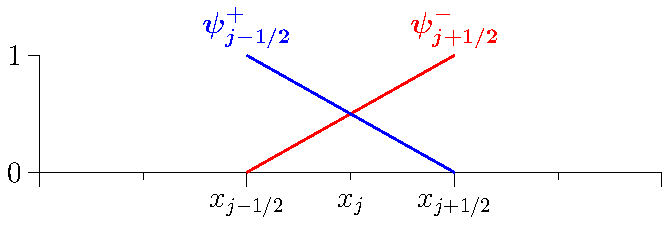
\includegraphics[width=0.8\textwidth]{./chp3/figures/P1.pdf}
	\caption{Discontinuous linear basis functions over a cell.}
	\label{fig:P1DiscBasis}
\end{figure}
From the basis functions $\psi$ we have the following representation for $h$ and $G$ in our FEM
\begin{subequations}
\begin{align}
\label{eqn:FEapproxtoh}
h &= \sum_j h^+_{j-1/2}\psi^+_{j-1/2}  + h^-_{j+1/2}\psi^-_{j+1/2}, \\
G &= \sum_j G^+_{j-1/2}\psi^+_{j-1/2}  + G^-_{j+1/2}\psi^-_{j+1/2}.
\label{eqn:FEapproxtoG}
\end{align}
\label{eqn:FEapproxtohG}
\end{subequations}


To calculate the flux and source terms of the evolution of $G$ equation \eqref{eqn:Serreconsconmom} we require a locally  calculated second-order approximation to the first derivative of $u$. To do this we require a quadratic representation of $u$ in each cell and since $u\in\mathbb{W}^{1,p}$, this representation will be continuous across the cell edges $x_{j \pm 1/2}$. Therefore, we use the continuous quadratic basis functions $\phi_{j-1/2} $ depicted in Figure \ref{fig:P2ContBasis}.

From the basis functions $\phi$ our basis function approximation to $u$ is
\begin{equation}
u = \sum_j u_{j-1/2}\phi_{j-1/2} + u_{j}\phi_{j} + u_{j+1/2}\phi_{j+1/2}.
\label{eqn:FEapproxtou}
\end{equation}

\begin{figure}
	\centering
	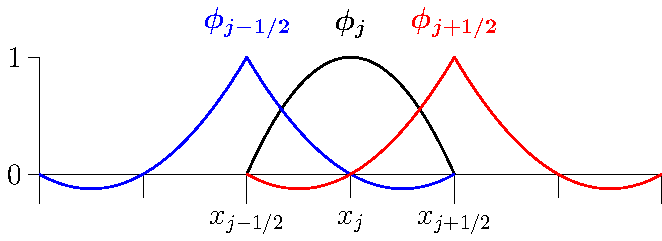
\includegraphics[width=0.8\textwidth]{./chp3/figures/P2.pdf}
	\caption{Continuous piecewise quadratic basis functions over a cell.}
	\label{fig:P2ContBasis}
\end{figure}

For the source term of the evolution of $G$ equation \eqref{eqn:Serreconsconmom} we require a local approximation to the second derivative of the bed that is second-order accurate. To allow for an appropriate second derivative of the bed profile, $b$ must be a member of $\mathbb{W}^{2,p}$ which is smoother than indicated by the elliptic equation \eqref{eqn:WeakFormDomain}. We choose the cubic basis functions $\gamma$ which are continuous across the cell edges, as the bed profile will be continuous. These basis functions are shown in Figure \ref{fig:P3ContBasis} and from them we get our basis function approximation to $b$
\begin{figure}
	\centering
	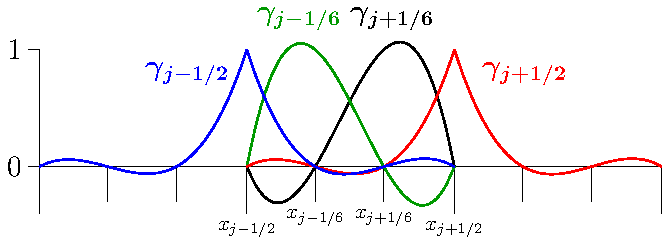
\includegraphics[width=0.8\textwidth]{./chp3/figures/P3.pdf}
	\caption{Continuous piecewise cubic basis functions over a cell.}
	\label{fig:P3ContBasis}
\end{figure}
\begin{equation}
b = \sum_j b_{j-1/2}\gamma_{j-1/2} + b_{j-1/6}\gamma_{j-1/6}  + b_{j+1/6}\gamma_{j+1/6} + b_{j+1/2}\gamma_{j+1/2}.
\label{eqn:FEapproxtob}
\end{equation}
With $b_{j-1/2}$ and $b_{j+1/2}$ being well defined as \eqref{eqn:FEVMbedrecon} imposes a unique reconstruction at the cell edges. 

\subsubsection{Calculation of Element-wise Matrices}
The integral equation \eqref{eq:elementwiseint} holds for all $\tau$. However, since our solution space has the basis functions $\phi$ it is sufficient to satisfy \eqref{eq:elementwiseint} for all $\phi$ to generate the solution. Since only the basis functions $\phi_{j-1/2}$, $\phi_{j}$ and $\phi_{j+1/2}$ are non-zero over the $j^{th}$ cell we can calculate the $j^{th}$ term in the sum \eqref{eq:elementwiseint} like so
\begin{multline}
\int_{x_{j-1/2} }^{{x_{j+1/2}}} \Bigg[  \left( uh \left(1 + \frac{\partial b}{\partial x}^2 \right)  - \frac{1}{2}h^2\frac{\partial b}{\partial x}  \frac{\partial u }{\partial x}  -  G \right) \begin{bmatrix}
\phi_{j-1/2}\\\phi_j \\\phi_{j+1/2}
\end{bmatrix}   \\ +  \left( \frac{1}{3}h^3  \frac{\partial {u}}{\partial x}    -     \frac{1}{2}h^2\frac{\partial b}{\partial x} u    \right) \frac{\partial}{\partial x}\left(\begin{bmatrix}
\phi_{j-1/2}\\\phi_j \\\phi_{j+1/2}
\end{bmatrix} \right) \Bigg]dx
\label{eqn:WeakFormElemXspace}
\end{multline}
where we use our finite element approximations for $h$ \eqref{eqn:FEapproxtoh}, $G$ \eqref{eqn:FEapproxtoG}, $u$ \eqref{eqn:FEapproxtou} and $b$ \eqref{eqn:FEapproxtob}. Because the basis functions over an element are just translations of the other basis functions, this integral can be generalised by moving to the $\xi$ space. The mapping from the $x$ space to the $\xi$ space is
\begin{equation*}
x = x_j + \xi \frac{\Delta x}{2}.
\end{equation*}
Making the change of variables from $x$ to $\xi$ in \eqref{eqn:WeakFormElemXspace} we get
\begin{multline*}
\frac{\Delta x}{2}\int_{-1 }^{1} \Bigg[  \left( uh \left(1 + \frac{4}{\Delta x^2}\frac{\partial b}{\partial \xi}^2 \right)  - \frac{2}{\Delta x^2} h^2 \frac{\partial b}{\partial \xi}  \frac{\partial u }{\partial \xi}  -  G \right) \begin{bmatrix}
\phi_{j-1/2}\\\phi_j \\\phi_{j+1/2}
\end{bmatrix}   \\ + \frac{4}{\Delta x^2} \left( \frac{1}{3}h^3 \frac{\partial {u}}{\partial \xi}    -     \frac{1}{2}h^2 \frac{\partial b}{\partial \xi} u    \right) \frac{\partial}{\partial \xi}\left(\begin{bmatrix}
\phi_{j-1/2}\\\phi_j \\\phi_{j+1/2}
\end{bmatrix} \right) \Bigg]d\xi.
\end{multline*}

We will demonstrate the rest of the process for the $uh$ term as an example and provide the remaining integrals in Appendix \ref{app:FEMIntegrals}. The $uh$ term is 
\begin{equation*}
\frac{\Delta x}{2}\int_{-1 }^{1}  uh \begin{bmatrix}
\phi_{j-1/2}\\\phi_j \\\phi_{j+1/2}
\end{bmatrix} d\xi.
\end{equation*}
Since the integral is computed over $\left[x_{j-1/2},x_{j+1/2}\right]$, there are only a few non-zero contributions from the finite element approximations to $h$ and $u$, so we have
\begin{multline*}
\frac{\Delta x}{2}\int_{-1 }^{1}  \left(u_{j-1/2}\phi_{j-1/2} + u_{j}\phi_{j} + u_{j+1/2}\phi_{j+1/2}\right) \\\left(h^+_{j-1/2}\psi^+_{j-1/2}  + h^-_{j+1/2}\psi^-_{j+1/2}\right) \begin{bmatrix}
\phi_{j-1/2}\\\phi_j \\\phi_{j+1/2}
\end{bmatrix} d\xi\\
=\frac{\Delta x}{2}\Bigg( h^+_{j-1/2} \int_{-1 }^{1} \psi^+_{j-1/2}  \begin{bmatrix}
\phi_{j-1/2} \phi_{j-1/2} & \phi_{j}  \phi_{j-1/2}  & \phi_{j+1/2} \phi_{j-1/2}\\\phi_{j-1/2} \phi_{j} & \phi_{j} \phi_{j} &  \phi_{j + 1/2} \phi_{j}\\\phi_{j+1/2} \phi_{j-1/2} &  \phi_{j+1/2} \phi_{j} & \phi_{j+1/2} \phi_{j+1/2}
\end{bmatrix} d\xi  \\ +  h^-_{j+1/2}\int_{-1 }^{1} \psi^-_{j+1/2} \begin{bmatrix}
\phi_{j-1/2} \phi_{j-1/2} & \phi_{j}  \phi_{j-1/2}  & \phi_{j+1/2} \phi_{j-1/2}\\\phi_{j-1/2} \phi_{j} & \phi_{j} \phi_{j} &  \phi_{j + 1/2} \phi_{j}\\\phi_{j+1/2} \phi_{j-1/2} &  \phi_{j+1/2} \phi_{j} & \phi_{j+1/2} \phi_{j+1/2}
\end{bmatrix} d\xi \Bigg) \\  \begin{bmatrix}
u_{j-1/2}\\u_j \\u _{j+1/2}
\end{bmatrix}.
\end{multline*}

Calculating the integrals of all the basis function combinations we get

\begin{multline}
\frac{\Delta x}{2}\int_{-1 }^{1}  uh \begin{bmatrix}
\phi_{j-1/2}\\\phi_j \\\phi_{j+1/2}
\end{bmatrix} d\xi =  \\  \frac{\Delta x}{2} \begin{bmatrix}
\frac{7}{30 } h^+_{j-1/2} + \frac{1}{30} h^-_{j+1/2} & \frac{4}{30 } h^+_{j-1/2}   & -\frac{1}{30 } h^+_{j-1/2} - \frac{1}{30} h^-_{j+1/2}\\\frac{4}{30 } h^+_{j-1/2} & \frac{16}{30 } h^+_{j-1/2} + \frac{16}{30} h^-_{j+1/2}&  \frac{4}{30} h^-_{j+1/2}\\ -\frac{1}{30 } h^+_{j-1/2} - \frac{1}{30} h^-_{j+1/2} &  \frac{4}{30 } h^-_{j+1/2} & \frac{1}{30 } h^+_{j-1/2} + \frac{7}{30} h^-_{j+1/2}
\end{bmatrix} \\  \begin{bmatrix}
u_{j-1/2}\\u_j \\u _{j+1/2}
\end{bmatrix}.
\end{multline}

\subsubsection{Assembly of the Global Matrix}
By combining all the matrices generated by the integral of each of the $u$ terms we get the $j^{th}$ cells contribution to the stiffness matrix $\matr{A}_j$. Likewise all the integrals of the remaining term $G\tau$ generate the vector $\vecn{g}_{j}$. Therefore, \eqref{eq:elementwiseint} can be rewritten as
\begin{equation}
\label{eqn:FEMElemMatrixJ}
\sum_j \matr{A}_j \begin{bmatrix}
u_{j-1/2}\\u_j \\u _{j+1/2}.
\end{bmatrix} = \sum_j \vecn{g}_j.
\end{equation}
This is a penta-diagonal matrix equation which can be solved by direct banded matrix solution techniques such as those of \citet{NumRecC-1996} to obtain
\begin{equation}
\vecn{\hat{u}} =\mathcal{G}\left( \vecn{\hat{h}}, \vecn{\hat{G}},\vecn{\hat{b}} \right) =   \matr{A}^{-1}\vecn{g}
\label{eqn:usolvefromGhb}
\end{equation}
as desired.
\subsection{Flux Across the Cell Interfaces}

We use Kurganovs method \cite{Kurganov-etal-2001-707} to calculate the flux across a cell interface. This method was employed because; it can handle discontinuities across the cell boundary and only requires an estimate of the maximum and minimum wave speeds. This is precisely the situation for the Serre equations which do not have an expression for the characteristics but do possess estimates on the maximum and minimum wave speeds \eqref{eqn:WaveVelocitiesBound}.

Only the calculation of the flux term $F_{j+1/2}$ is demonstrated as the process to calculate the flux term $F_{j-1/2}$ is identical but with different cells. For a general quantity $q$, Kurganov's method \cite{Kurganov-etal-2001-707} is
\begin{equation}\label{eqn:HLL_flux}
F_{j+\frac{1}{2}} = \dfrac{a^+_{j+\frac{1}{2}} f\left(q^-_{j+\frac{1}{2}}\right) - a^-_{j+\frac{1}{2}} f\left(q^+_{j+\frac{1}{2}}\right)}{a^+_{j+\frac{1}{2}} - a^-_{j+\frac{1}{2}}}  + \dfrac{a^+_{j+\frac{1}{2}} \, a^-_{j+\frac{1}{2}}}{a^+_{j+\frac{1}{2}} - a^-_{j+\frac{1}{2}}} \left [ q^+_{j+\frac{1}{2}} - q^-_{j+\frac{1}{2}} \right ]
\end{equation}

where $a^+_{j+\frac{1}{2}}$ and $a^-_{j+\frac{1}{2}}$ are given by the wave speed bounds. Applying the wave speed bounds \eqref{eqn:WaveVelocitiesBound} we obtain

\begin{align}
a^-_{j+\frac{1}{2}} &= \min\left\lbrace 0\;,\;  u^-_{j + 1/2} - \sqrt{g h^-_{j + 1/2}}  \;,\;u^+_{j + 1/2} - \sqrt{g h^+_{j + 1/2}} \right\rbrace  ,\\
a^+_{j+\frac{1}{2}} &= \max\left\lbrace 0 \;,\;  u^-_{j + 1/2} + \sqrt{g h^-_{j + 1/2}}  \;,\;u^+_{j + 1/2} + \sqrt{g h^+_{j + 1/2}} \right\rbrace .
\label{eqn:WaveSpeedBoundsFluxApprox}
\end{align}

The flux functions $f(q^-_{j+\frac{1}{2}})$ and $f(q^+_{j+\frac{1}{2}})$ are evaluated using the reconstructed values of the $j^{th}$ and $(j+1)^{th}$ cell respectively. From the continuity equation \eqref{eqn:FullSerreConMass} we have
\begin{align*}
f\left(h^-_{j+\frac{1}{2}}\right) &= u^-_{j + 1/2}  h^-_{j + 1/2}   ,\\
f\left(h^+_{j+\frac{1}{2}}\right) &= u^+_{j + 1/2}  h^+_{j + 1/2}  .
\end{align*}

For the evolution of $G$ equation \eqref{eqn:Serreconsconmom} we have 
\begin{subequations}
\begin{align}
f\left(G^-_{j+\frac{1}{2}}\right) &=  u^-_{j + 1/2} G^-_{j + 1/2}  + \frac{g}{2}\left(h^-_{j + 1/2} \right)^2 - \frac{2}{3}\left(h^-_{j + 1/2}\right)^3 \left[\left(\frac{\partial {u}}{\partial x} \right)^-_{j + 1/2} \right]^2 \nonumber\\ &+ \left(h^-_{j + 1/2}\right)^2 u^-_{j + 1/2} \left(\frac{\partial {u}}{\partial x} \right)^-_{j + 1/2} \left(\frac{\partial b}{\partial x} \right)^-_{j + 1/2}  ,\\ \nonumber \\
f\left(G^+_{j+\frac{1}{2}}\right) &= u^+_{j + 1/2} G^+_{j + 1/2}  + \frac{g}{2}\left(h^+_{j + 1/2} \right)^2 - \frac{2}{3}\left(h^+_{j + 1/2}\right)^3 \left[\left(\frac{\partial {u}}{\partial x} \right)^+_{j + 1/2} \right]^2 \nonumber\\ &+ \left(h^+_{j + 1/2}\right)^2 u^+_{j + 1/2} \left(\frac{\partial {u}}{\partial x} \right)^+_{j + 1/2} \left(\frac{\partial b}{\partial x} \right)^+_{j + 1/2}.
\end{align}
\label{eqn:FluxIrrotNum}
\end{subequations}

During the reconstruction process $h^+_{j - 1/2}$, $h^-_{j + 1/2}$, $G^+_{j - 1/2}$, $G^-_{j + 1/2}$ \eqref{eqn:ReconforhwG} were calculated, and the FEM provided $u^\pm_{j+1/2} = u_{j+1/2}$; because $u$ is continuous across the cell boundaries. Therefore, approximations to $\left(\dfrac{\partial {b}}{\partial x} \right)^\pm_{j + 1/2}$ and $\left(\dfrac{\partial {u}}{\partial x} \right)^\pm_{j + 1/2}$ are required to calculate the flux \eqref{eqn:FluxIrrotNum}. 

\subsubsection{Calculation of Derivatives}
To calculate the derivatives in $u$ and $b$ we use the basis function approximation to these quantities in the FEM. For $u$ we have the quadratic $P_j^u(x)$ that passes through $u_{j-1/2}$, $u_j$ and $u_{j+1/2}$ while for $b$ we have the cubic $P_j^b(x)$ that passes through $b_{j-1/2}$, $b_{j-1/6}$, $b_{j+1/6}$ and $b_{j+1/2}$. So we have 
\begin{subequations}
	\begin{align}
	P^u_j(x) &= p^u_0 \left(x - x_j\right)^2 + p^u_1 \left(x - x_j\right) + p^u_2, \\
	P^b_j(x) &= p^b_0 \left(x - x_j\right)^3 + p^b_1 \left(x - x_j\right)^2 + p^b_2 \left(x - x_j\right)  + p^b_3,
	\end{align}
	\label{eqn:Polyforuandbcell}
\end{subequations}
By forcing the polynomials to pass through these reconstructed values we get that for $P^u_j(x)$
\begin{align*}
p^u_0 &=  \dfrac{u_{j-1/2} - 2u_j + u_{j+1/2}}{2 \Delta x^2},\\
p^u_1 &=  \dfrac{-u_{j-1/2} + u_{j+1/2}}{\Delta x},\\
p^u_2 &=  u_j.
\end{align*}
While for $P^b_j(x)$ we get
\begin{align*}
p^b_0 &=  \dfrac{-9b_{j-1/2} + 27b_{j-1/6} - 27 b_{j+1/6} + 9b_{j+1/2}}{2 \Delta x^3},\\ \\
p^b_0 &=  \dfrac{9b_{j-1/2} - 9b_{j-1/6} - 9b_{j+1/6} + 9b_{j+1/2}}{4 \Delta x^2},\\ \\ 
p^b_0 &=  \dfrac{b_{j-1/2} - 27b_{j-1/6} + 27 b_{j+1/6} - b_{j+1/2}}{8 \Delta x},\\\\
p^b_0 &=  \dfrac{-b_{j-1/2}  + 9b_{j-1/6} + 9 b_{j+1/6} - b_{j+1/2}}{16}.
\end{align*}
Taking the derivative of the polynomials \eqref{eqn:Polyforuandbcell} we get
	\begin{align*}
	\frac{\partial }{\partial x}P^u_j(x) &= 2p^u_0 \left(x - x_j\right) + p^u_1, \\
	\frac{\partial }{\partial x}P^b_j(x) &= 3p^b_0 \left(x - x_j\right)^2 + 2p^b_1 \left(x - x_j\right) + p^b_2.
	\end{align*}
This gives a second-order approximation to the derivative of $u$ and $b$ at $x_{j+1/2}$ for the $j^{th}$ cell. The process for the $(j+1)^{th}$ cell is the same and we get 
\begin{subequations}
	\begin{align}
	\left(\dfrac{\partial {u}}{\partial x} \right)^-_{j + 1/2} &= \frac{\partial }{\partial x}P^u_j(x_{j+1/2}),  \\
	\left(\dfrac{\partial {u}}{\partial x} \right)^+_{j + 1/2} &= \frac{\partial }{\partial x}P^u_{j+1}(x_{j+1/2}),  \\
	\left(\dfrac{\partial {b}}{\partial x} \right)^-_{j + 1/2} &= \frac{\partial }{\partial x}P^b_j(x_{j+1/2}), \\
	\left(\dfrac{\partial {b}}{\partial x} \right)^+_{j + 1/2} &= \frac{\partial }{\partial x}P^b_{j+1}(x_{j+1/2}). 	\end{align}
	\label{eqn:dbduRecon}
\end{subequations}

Therefore, we possess all the terms need to calculate the approximation to the flux \eqref{eqn:HLL_flux} for both the continuity and evolution of $G$ equation, as desired. However, to ensure that the FEVM is well balanced and recovers the lake at rest steady state solution, these fluxes must be modified.

\subsubsection{Well Balancing}
To recover the lake at rest steady state solution we follow the work of \citet{Klein-etal-2004-2050}, who accomplished this for the SWWE. It was demonstrated that this process could also be extended to the Serre equations \cite{Pitt-J-2014}. To enforce well balancing the reconstruction of $h$ is modified at the cell edges in the following way; first calculate
\begin{align}
\dot{b}^-_{j+1/2} = w^-_{j+1/2} - h^-_{j+1/2} & &\text{and}& &\dot{b}^+_{j+1/2} = w^+_{j+1/2} - h^+_{j+1/2}.
\label{eqn:BedReDefWmH}
\end{align}
Find the maximum
\begin{align*}
\grave{b}_{j+1/2} = \max\left\lbrace\dot{b}^-_{j+1/2} , \dot{b}^+_{j+1/2} \right\rbrace
\end{align*}
then define
\begin{subequations}
\begin{align}
\grave{h}^-_{j+1/2} &= \max\left\lbrace 0, w^-_{j+1/2} - \grave{b}_{j+1/2}  \right\rbrace, \\  \grave{h}^+_{j+1/2} &= \max\left\lbrace 0, w^+_{j+1/2} - \grave{b}_{j+1/2} \right\rbrace.
\end{align}
\label{eqn:ModifiedHValue}
\end{subequations}
This generates the vector $\vecn{\grave{h}}$
\begin{equation*}
\vecn{\grave{h}}= \begin{bmatrix}
\grave{h}^+_{-1/2} \\ h_0 \\ \grave{h}^-_{1/2}  \\ \grave{h}^+_{1/2}  \\ \vdots  \\ h_m  \\ \grave{h}^-_{m + 1/2} \end{bmatrix}
\end{equation*}
which we use to calculate the flux term $F_{j+1/2}$ in \eqref{eqn:HLL_flux} for both the continuity \eqref{eqn:FullSerreConMass} and evolution of $G$ \eqref{eqn:Serreconsconmom} equation. Applying the same process but with different cells we obtain $F_{j-1/2}$ and we have
\begin{subequations}
\begin{align}	
F_{j-1/2} &=\mathcal{F}_{j-1/2} \left(\vecn{\grave{h}}, \vecn{\hat{G}},\vecn{\hat{b}}, \vecn{\hat{u}}  \right),\\
F_{j+1/2} &=\mathcal{F}_{j+1/2} \left(\vecn{\grave{h}}, \vecn{\hat{G}},\vecn{\hat{b}}, \vecn{\hat{u}}  \right)
\label{eqn:FluxFEVM}
\end{align}
\end{subequations}


for both the continuity and evolution of $G$ equation as desired.

\subsection{Source Terms}
The Serre equations in conservative form \eqref{eqn:FullSerreCon} contain a flux term and a source term, to treat this numerically we use a first-order splitting method. This requires an approximation to the source term at the cell centre $x_j$ which we denote as $S_j$. Since the continuity equation \eqref{eqn:FullSerreConMass} has no source term, we will just present the calculation of the source term for the evolution of $G$ equation \eqref{eqn:Serreconsconmom}.

Following the work of \citet{Klein-etal-2004-2050}, we split our approximation to $S_j$ into the centred source term $S_{ci}$ and the corrective interface source terms $S^{-}_{j + \frac{1}{2}}$ and $S^{+}_{j + \frac{1}{2}}$.
Where $S_{ci}$ is the naive source term approximation and $S^{-}_{j + \frac{1}{2}}$ and $S^{+}_{j + \frac{1}{2}}$ are correction terms that ensure that the flux and source term cancel for the lake at rest steady state. 

We calculate the centred source term using
\begin{equation*}
 S_{ci} = -\frac{1}{2}\left(h_j\right)^2 {u_j}\left( \frac{\partial {u}}{\partial x} \right)_j \left(\frac{\partial^2 b}{\partial x^2} \right)_j  + h_j \left(u_j\right)^2 \left(\frac{\partial b}{\partial x}\right)_j \left(\frac{\partial^2 b}{\partial x^2}\right)_j - gh_j\left(\frac{\partial b}{\partial x}\right)_j.
\end{equation*}
Where we use $h_j$ from the reconstruction process \eqref{eqn:ReconforhwG} and $u_j$ from the solution of the elliptic equation \eqref{eqn:usolvefromGhb}. To calculate the derivatives we employ our polynomial representations of $u$ and $b$ inside a cell. However, to ensure that the terms cancel properly for a lake at rest we modify our approximation to $\dfrac{\partial b}{\partial x}$ to use $\dot{b}^-_{j+1/2}$ and $\dot{b}^+_{j+1/2}$ from \eqref{eqn:BedReDefWmH}. Therefore, the following approximations are used to calculate $S_{ci}$
\begin{subequations}
	\begin{align}
	\left(\dfrac{\partial {u}}{\partial x} \right)_{j} &= \frac{\partial }{\partial x}P^u_j(x_{j}),  \\
\left(\dfrac{\partial {b}}{\partial x} \right)_{j} &=  \frac{\dot{b}^-_{j+1/2} - \dot{b}^+_{j-1/2}}{\Delta x} , \\	
	\left(\dfrac{\partial^2 {b}}{\partial x^2} \right)_{j} &= \frac{\partial^2 }{\partial x^2}P^b_j(x_{j}).
	\end{align}
	\label{eqn:dbduReconSource}
\end{subequations}

The corrective interface source terms are
	\begin{align*}
	 S^{-}_{j + \frac{1}{2}} &=  \frac{g}{2} \left(\grave{h}^{-}_{j + \frac{1}{2}} \right)^2 - \frac{g}{2} \left(h^{-}_{j + \frac{1}{2}} \right)^2, \\ \\
	  S^{+}_{j - \frac{1}{2}} &=  \frac{g}{2} \left(h^{+}_{j - \frac{1}{2}}\right)^2 - \frac{g}{2}\left(\grave{h}^{+}_{j - \frac{1}{2}}\right)^2 .	 
	\end{align*}
Which makes use of $h^{-}_{j + \frac{1}{2}}$ and $h^{+}_{j + \frac{1}{2}}$ obtained from the reconstruction \eqref{eqn:ReconforhwG} and the modified values $\grave{h}^{-}_{j + \frac{1}{2}}$ and $\grave{h}^{+}_{j + \frac{1}{2}}$ from \eqref{eqn:ModifiedHValue}. Combining the centred and interface source terms our approximation to the source term for the evolution of $G$ equation is
%h' in function []?[]
\begin{equation}
S_j = \mathcal{S}_j\left( \vecn{\hat{h}},\vecn{\grave{h}},\vecn{\hat{w}},\vecn{\hat{b}}, \vecn{\hat{u}}  \right) =  S^{-}_{j + \frac{1}{2}} + \Delta x S_{ci} + S^{+}_{j - \frac{1}{2}}.
\label{eqn:SourceTerm}
\end{equation}


\subsection{Update Cell Averages}
We use the forward Euler approximation to approximate the time derivatives and obtain an update formula for the cell averages. Additionally we employ a fractional step method to split the flux term and source term part of the Serre equations written in conservative form \eqref{eqn:FullSerreCon}. This results in the following time-stepping method that is first-order accurate in time
\begin{align*}
\overline{q}'_j &= \overline{q}^{n}_j + \frac{\Delta t}{\Delta x} \left(F_{j+\frac{1}{2}} - F_{j-\frac{1}{2}}\right), \\
\overline{q}^{n+1}_j &= \overline{q}'_j + \frac{\Delta t}{\Delta x} S_j
\end{align*}
where $F_{j+\frac{1}{2}}$, $F_{j-\frac{1}{2}}$ and $S_j$ are all calculated using the quantities at time $t^n$. Therefore, this method can be condensed into
\begin{align}
\overline{q}^{n+1}_j &= \overline{q}^{n}_j + \frac{\Delta t}{\Delta x} \left(F_{j+\frac{1}{2}} - F_{j-\frac{1}{2}} + S_j\right).
\label{eqn:UpdateMethod}
\end{align}

\subsection{Second-Order SSP Runge-Kutta Method}
To increase the order of accuracy in time we employ the strong stability preserving Runge-Kutta method \cite{Gottlieb-etal-2003-89} which is a convex combination of multiple first-order time steps \eqref{eqn:UpdateMethod} in the following way
\begin{subequations}
\begin{align}
\overline{q}_j' &= \overline{q}^{n}_j + \frac{\Delta t}{\Delta x} \left(F_{j+\frac{1}{2}} - F_{j-\frac{1}{2}} + S_j\right),\\
\overline{q}_j'' &= \overline{q}_j' + \frac{\Delta t}{\Delta x} \left(F_{j+\frac{1}{2}}' - F_{j-\frac{1}{2}}'  + S_j' \right), \\
\overline{q}^{n+1}_j &= \frac{1}{2} \left( \overline{q}^n_j +  \overline{q}_j'' \right).
\end{align}
\label{eqn:SSPRKStep1}
\end{subequations}
%TVD no oscillations introduced by the particular method
This results in a time stepping method that preserves the stability of the first-order method \eqref{eqn:UpdateMethod} and is second-order accurate in time. Since all the spatial approximations are second-order accurate, the steps (I-VI) should result in a second-order accurate FEVM for the Serre equations, as desired. 

\setcounter{subsection}{0}
\renewcommand{\thesubsection}{\thechapter.\arabic{section}.\arabic{subsection}} 

\section{CFL condition}
To ensure the stability of our FEVM we use the Courant-Friedrichs-Lewy (CFL) condition \cite{Courant-etal-1967-215} which is necessary for stability. The CFL condition ensures that time steps are small enough so that information is only transferred between neighbouring cells. For the Serre equations the CFL condition is 
\begin{equation}
\Delta t \le \frac{Cr }{\max_{j} \left\lbrace a^\pm_{j+1/2} \right\rbrace} \Delta x
\label{eqn:CFLcond}
\end{equation}
where $a^\pm_{j+1/2} $ are the wavespeed bounds used in Kurganovs flux approximation \eqref{eqn:WaveSpeedBoundsFluxApprox} and $0\le Cr \le 1$ is the Courant number. Typically, we use the conservative $Cr = 0.5$ for our numerical experiments. 

\section{Boundary Conditions}
To numerically model the Serre equations over finite spatial domains we must enforce boundary conditions at the left and right edge of the domain; $x_{-1/2}$ and $x_{m+1/2}$ respectively. We have only developed Dirichlet boundary conditions for the FEVM, which we enforce using ghost cells located outside the domain boundaries. These ghost cells contain the complete representation of their respective quantities over the cell. For $h$, $w$, $G$ and $u$ only one ghost cell at each boundary is required, while for $b$ we require two ghost cells at each boundary. We therefore have ghost cells with the following associated quantities

\begin{align*}
&\vecn{\hat{h}}_{-1} = \begin{bmatrix}
h^+_{-3/2} \\ h_{-1} \\ h^-_{-1/2}\end{bmatrix},&\vecn{\hat{h}}_{m+1} = \begin{bmatrix}
h^+_{m+1/2} \\ h_{m+1} \\h^-_{m+3/2}\end{bmatrix}&, \\
&\vecn{\hat{w}}_{-1} = \begin{bmatrix}
w^+_{-3/2} \\ w_{-1} \\ w^-_{-1/2}\end{bmatrix},&\vecn{\hat{w}}_{m+1} = \begin{bmatrix}
w^+_{m+1/2} \\ w_{m+1} \\ w^-_{m+3/2}\end{bmatrix}&, \\
&\vecn{\hat{G}}_{-1} = \begin{bmatrix}
G^+_{-3/2} \\ G_{-1} \\ G^-_{-1/2}\end{bmatrix},&\vecn{\hat{G}}_{m+1} = \begin{bmatrix}
G^+_{m+1/2} \\ G_{m+1} \\ G^-_{m+3/2}\end{bmatrix}&, \\
&\vecn{\hat{u}}_{-1} = \begin{bmatrix}
u_{-3/2} \\ u_{-1} \\ u_{-1/2}\end{bmatrix},&\vecn{\hat{u}}_{m+1} = \begin{bmatrix}
u_{m+1/2} \\ u_{m+1} \\ u_{m+3/2}\end{bmatrix}&
\end{align*}
\begin{align*}
\vecn{\hat{b}}_{-2} = \begin{bmatrix}
b_{-5/2} \\ b_{-13/6} \\ b_{-11/6} \\ b_{-3/2}\end{bmatrix}&, &\vecn{\hat{b}}_{-1} = \begin{bmatrix}
b_{-3/2} \\ b_{-7/6} \\ b_{-5/6} \\ b_{-1/2}\end{bmatrix}&, &\vecn{\hat{b}}_{m+1} = \begin{bmatrix}
b_{m+1/2} \\ b_{m+5/6} \\ b_{m+7/6} \\ b_{m+3/2}\end{bmatrix}&, &\vecn{\hat{b}}_{m+2} = \begin{bmatrix}
b_{m+3/2} \\ b_{m+11/6} \\ b_{m+13/6} \\ b_{m+5/2}\end{bmatrix}.
\end{align*}

To ensure that the solution of $u$ by \eqref{eqn:usolvefromGhb} agrees with the boundary conditions $\vecn{\hat{u}}_{-1}$ and $\vecn{\hat{u}}_{m}$ the element matrices $\matr{A}_0$ and $\matr{A}_m$ and vectors $\vecn{g}_0$ and $\vecn{g}_m$ must be modified in the following way 

\begin{align}
\matr{A}_{0} = 
\begin{bmatrix}
1 &0 &0 \\
a_{21} & a_{22} & a_{23} \\
a_{31} & a_{32} & a_{33} \\
\end{bmatrix} &,& \vecn{g}_{0} = \begin{bmatrix}
u_{-1/2} \\
g_1 \\
g_2 \\
\end{bmatrix},\\
\matr{A}_{m} = 
\begin{bmatrix}
a_{11} & a_{12} & a_{13} \\
a_{21} & a_{22} & a_{23} \\
0 & 0 & 1 \\
\end{bmatrix} &,& \vecn{g}_{m} = \begin{bmatrix}
g_0\\
g_1 \\
u_{m+1/2} \\
\end{bmatrix}.
\end{align}
These are then combined with the other element contributions in the global matrix \eqref{eqn:FEMElemMatrixJ}.


\section{Dry Beds}
%Better description of what this method is trying to achieve:
% 1. Matrix solver should be able to handle '0' values in the band, it does this by raising pivots to be a very small number, p_tol

%2. Want to have h = 0 when below h_tol

% 2.Introduces small error when h is large -> h_{base}

%[]---[] Desingularisation Transform, Kurganov, other papers, denomintor added to to keep away from 0, choices of h0 h1 effect the errors in u but deccrease artificial error added to method
%think about G approx uh

Dry beds are handled adequately by all steps of our FEVM in their current form, except the FEM solution for $u$. For the FEM a dry bed presents two issues; when $h=0$ the stiffness matrix will become singular, and when $h$ is small $u$ may become quite large leading to instabilities. 

In previous work \cite{Zoppou-etal-2017} direct banded matrix solvers such as the Thomas algorithm were employed to solve \eqref{eqn:usolvefromGhb}, however such methods rely on non-singular matrices and so are unsuitable for dry beds. To deal with this an LU decomposition algorithm by \citet{NumRecC-1996} was used. This algorithm solves banded matrix problems using an LU decomposition with partial pivoting, which inserts small non-zero pivots when their value is below some tolerance value $p_{tol}$. It does this while also keeping the banded matrix structure, and so is not as memory intensive as a standard $LU$ decomposition. This results in a FEM that allows for $h=0$, but still faces the problem of large $u$ values when $h$ is small. 

To deal with large $u$ values we restricted our solution of the FEM for $u$ to cells where $\overline{h}_j> h_{tol}$ and modified our approximation to $h^+_{j-1/2}$ and $h^-_{j+1/2}$ in our stiffness matrix. To restrict the domain of our solution we search through the domain at the beginning of each first-order step and identify  wet regions where $\overline{h}_j \ge h_{tol}$ and dry regions where $\overline{h}_j < h_{tol}$. In the dry regions we set $h$, $G$ and $u$ to be zero uniformly over the cell. In the wet regions we solve the FEM with the appropriate boundary conditions and the following modifications to $h^+_{j-1/2}$ and $h^-_{j+1/2}$

\begin{subequations}
\begin{align}
h^+_{j-1/2} & = h^+_{j-1/2} \left(\frac{ h^+_{j-1/2}  + h_{base}}{h^+_{j-1/2} + h_{tol}}\right) , \\ \nonumber\\
h^-_{j+1/2} & = h^-_{j+1/2} \left(\frac{ h^-_{j+1/2}  + h_{base}}{h^-_{j+1/2} + h_{tol}}\right).
\end{align} 
\end{subequations}
%mention G going to 0.
Where on the right hand side we mean $h^+_{j-1/2}$ and $h^-_{j+1/2}$ as calculated from the reconstruction \eqref{eqn:ReconforhwG}. This modification ensures that as $h \rightarrow 0$ and correspondingly $G\rightarrow 0 $ then $u \rightarrow 0$ by increasing the size of $h$ in the stiffness matrix. 

Typically we had $p_{tol} = 10^{-20}$, $h_{tol} = 10^{-12}$ and $h_{base} = 10^{-8}$ which allowed for a stable calculation of $u$ in the presence of dry beds and small water depths. While the accuracy of the calculation of $u$ by the FEM was maintained when the water depth is large compared to $h_{tol}$ and $h_{base}$.

%[]